\documentclass{standalone}

\usepackage{tikz}
\usetikzlibrary{arrows}
\usetikzlibrary{decorations.markings}
\usetikzlibrary{calc}

\begin{document}

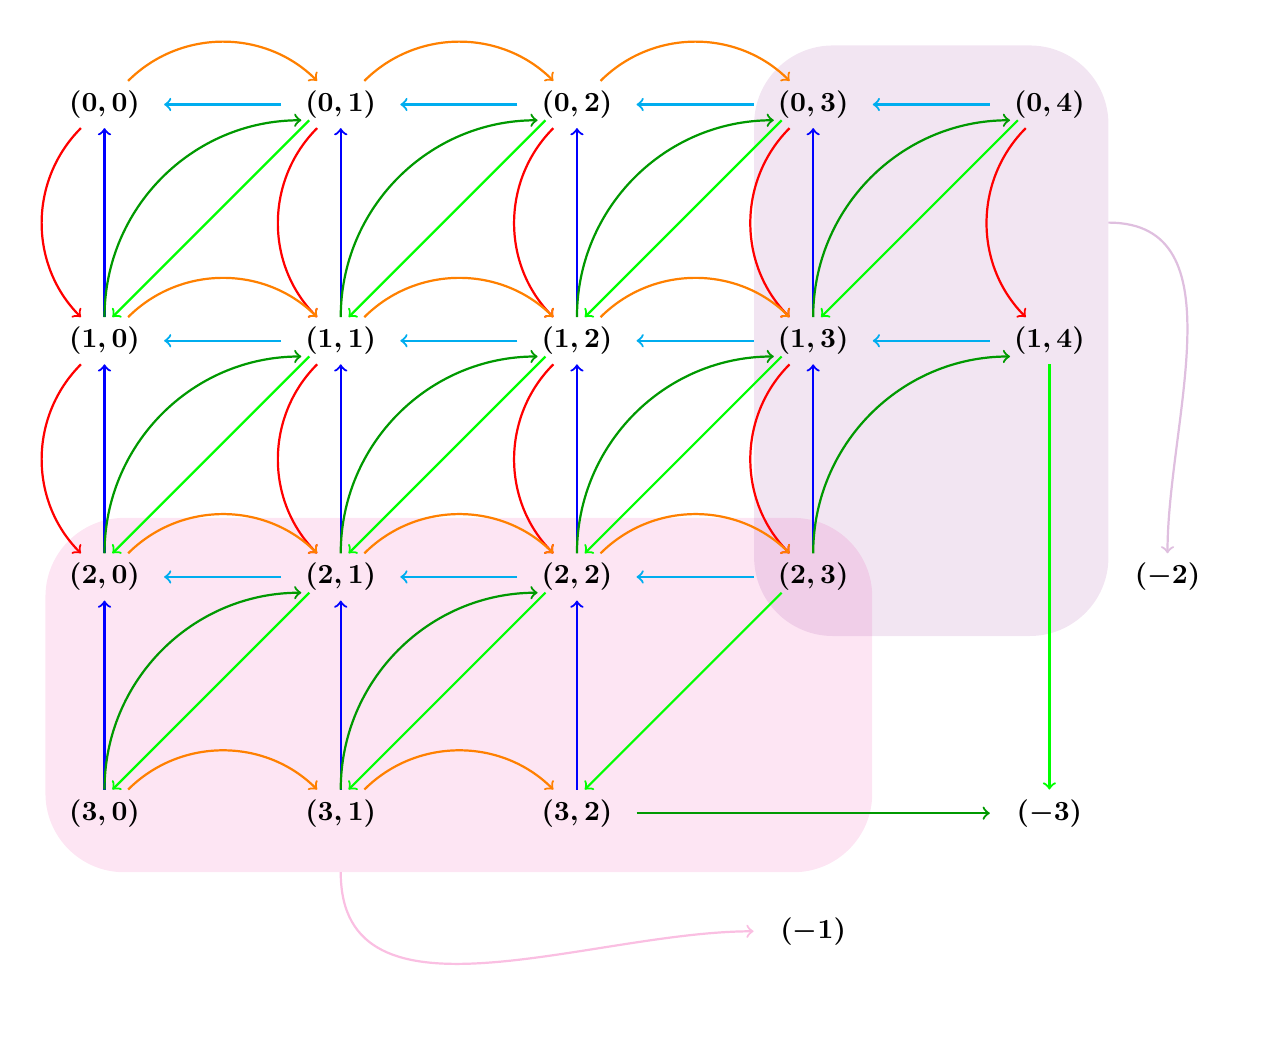
\begin{tikzpicture}
    
    \draw[rounded corners=10mm,fill=magenta, fill opacity=0.1, draw=none] (-0.75, -9.75) rectangle (9.75, -5.25);
    \draw[rounded corners=10mm,fill=violet, fill opacity=0.1, draw=none] (8.25, -6.75) rectangle (12.75, 0.75);

    \tikzstyle{state}=[minimum width=1.5cm, font=\boldmath];
    % First row
    \node (00) at (0,0) [state] {$(0,0)$};
    \node (01) at ($(00)+(3,0)$) [state] {$(0,1)$};
    \node (02) at ($(01)+(3,0)$) [state] {$(0,2)$};
    \node (03) at ($(02)+(3,0)$) [state] {$(0,3)$};
    \node (04) at ($(03)+(3,0)$) [state] {$(0,4)$};

    % Second row
    \node (10) at ($(00)+(0,-3)$) [state] {$(1,0)$};
    \node (11) at ($(10)+(3,0)$) [state] {$(1,1)$};
    \node (12) at ($(11)+(3,0)$) [state] {$(1,2)$};
    \node (13) at ($(12)+(3,0)$) [state] {$(1,3)$};
    \node (14) at ($(13)+(3,0)$) [state] {$(1,4)$};

    % Third row
    \node (20) at ($(10)+(0,-3)$) [state] {$(2,0)$};
    \node (21) at ($(20)+(3,0)$) [state] {$(2,1)$};
    \node (22) at ($(21)+(3,0)$) [state] {$(2,2)$};
    \node (23) at ($(22)+(3,0)$) [state] {$(2,3)$};

    % Fourth row
    \node (30) at ($(20)+(0,-3)$) [state] {$(3,0)$};
    \node (31) at ($(30)+(3,0)$) [state] {$(3,1)$};
    \node (32) at ($(31)+(3,0)$) [state] {$(3,2)$};

    \node (-3) at ($(23)+(3,-3)$) [state] {$(-3)$};
    \node (-1) at ($(32)+(3,-1.5)$) [state] {$(-1)$};
    \node (-2) at ($(14)+(1.5,-3)$) [state] {$(-2)$};

    % Transitions
    % Arrivals
    \draw[draw=red] (00) edge[out=-135,in=135,->,thick] (10);
    \draw[draw=red] (01) edge[out=-135,in=135,->,thick] (11);
    \draw[draw=red] (02) edge[out=-135,in=135,->,thick] (12);
    \draw[draw=red] (03) edge[out=-135,in=135,->,thick] (13);
    \draw[draw=red] (04) edge[out=-135,in=135,->,thick] (14);

    \draw[draw=red] (10) edge[out=-135,in=135,->,thick] (20);
    \draw[draw=red] (11) edge[out=-135,in=135,->,thick] (21);
    \draw[draw=red] (12) edge[out=-135,in=135,->,thick] (22);
    \draw[draw=red] (13) edge[out=-135,in=135,->,thick] (23);

    \draw[draw=orange] (00) edge[out=45,in=135,->,thick] (01);
    \draw[draw=orange] (01) edge[out=45,in=135,->,thick] (02);
    \draw[draw=orange] (02) edge[out=45,in=135,->,thick] (03);

    \draw[draw=orange] (10) edge[out=45,in=135,->,thick] (11);
    \draw[draw=orange] (11) edge[out=45,in=135,->,thick] (12);
    \draw[draw=orange] (12) edge[out=45,in=135,->,thick] (13);

    \draw[draw=orange] (20) edge[out=45,in=135,->,thick] (21);
    \draw[draw=orange] (21) edge[out=45,in=135,->,thick] (22);
    \draw[draw=orange] (22) edge[out=45,in=135,->,thick] (23);

    \draw[draw=orange] (30) edge[out=45,in=135,->,thick] (31);
    \draw[draw=orange] (31) edge[out=45,in=135,->,thick] (32);

    % % First Station Service and exit
    \draw[blue] (00) edge[<-,thick] (10);
    \draw[blue] (01) edge[<-,thick] (11);
    \draw[blue] (02) edge[<-,thick] (12);
    \draw[blue] (03) edge[<-,thick] (13);

    \draw[blue] (10) edge[<-,thick] (20);
    \draw[blue] (11) edge[<-,thick] (21);
    \draw[blue] (12) edge[<-,thick] (22);
    \draw[blue] (13) edge[<-,thick] (23);

    \draw[blue] (20) edge[<-,thick] (30);
    \draw[blue] (21) edge[<-,thick] (31);
    \draw[blue] (22) edge[<-,thick] (32);

    % Second station service and exit
    \draw[draw=cyan] (04) edge[->,thick] (03);
    \draw[draw=cyan] (03) edge[->,thick] (02);
    \draw[draw=cyan] (02) edge[->,thick] (01);
    \draw[draw=cyan] (01) edge[->,thick] (00);

    \draw[draw=cyan] (14) edge[->,thick] (13);
    \draw[draw=cyan] (13) edge[->,thick] (12);
    \draw[draw=cyan] (12) edge[->,thick] (11);
    \draw[draw=cyan] (11) edge[->,thick] (10);

    \draw[draw=cyan] (23) edge[->,thick] (22);
    \draw[draw=cyan] (22) edge[->,thick] (21);
    \draw[draw=cyan] (21) edge[->,thick] (20);

    % 1st station service and transition
    \draw[draw=green!60!black] (30) edge[out=90,in=180,->,thick] ($(21)+(-0.5,-0.2)$);
    \draw[draw=green!60!black] (20) edge[out=90,in=180,->,thick] ($(11)+(-0.5,-0.2)$);
    \draw[draw=green!60!black] (10) edge[out=90,in=180,->,thick] ($(01)+(-0.5,-0.2)$);

    \draw[draw=green!60!black] (31) edge[out=90,in=180,->,thick] ($(22)+(-0.5,-0.2)$);
    \draw[draw=green!60!black] (21) edge[out=90,in=180,->,thick] ($(12)+(-0.5,-0.2)$);
    \draw[draw=green!60!black] (11) edge[out=90,in=180,->,thick] ($(02)+(-0.5,-0.2)$);

    \draw[draw=green!60!black] (22) edge[out=90,in=180,->,thick] ($(13)+(-0.5,-0.2)$);
    \draw[draw=green!60!black] (12) edge[out=90,in=180,->,thick] ($(03)+(-0.5,-0.2)$);

    \draw[draw=green!60!black] (13) edge[out=90,in=180,->,thick] ($(04)+(-0.5,-0.2)$);
    \draw[draw=green!60!black] (23) edge[out=90,in=180,->,thick] ($(14)+(-0.5,-0.2)$);

    % 2ns station service and transition
    \draw[draw=green] ($(21)+(-0.4,-0.2)$) edge[->,thick] ($(30)+(0.1,0.3)$);
    \draw[draw=green] ($(11)+(-0.4,-0.2)$) edge[->,thick] ($(20)+(0.1,0.3)$);
    \draw[draw=green] ($(01)+(-0.4,-0.2)$) edge[->,thick] ($(10)+(0.1,0.3)$);

    \draw[draw=green] ($(22)+(-0.4,-0.2)$) edge[->,thick] ($(31)+(0.1,0.3)$);
    \draw[draw=green] ($(12)+(-0.4,-0.2)$) edge[->,thick] ($(21)+(0.1,0.3)$);
    \draw[draw=green] ($(02)+(-0.4,-0.2)$) edge[->,thick] ($(11)+(0.1,0.3)$);

    \draw[draw=green] ($(13)+(-0.4,-0.2)$) edge[->,thick] ($(22)+(0.1,0.3)$);
    \draw[draw=green] ($(03)+(-0.4,-0.2)$) edge[->,thick] ($(12)+(0.1,0.3)$);

    \draw[draw=green] ($(04)+(-0.4,-0.2)$) edge[->,thick] ($(13)+(0.1,0.3)$);
    \draw[draw=green] ($(23)+(-0.4,-0.2)$) edge[->,thick] ($(32)+(0.1,0.3)$);

    % To deadlock -3
    \draw[draw=green] (14) edge[->,thick] (-3);
    \draw[draw=green!60!black] (32) edge[->,thick] (-3);

    % To deadlock -2
    \draw[draw=magenta!25] ($(31)+(0,-0.75)$) edge[out=-90,in=180, ->, thick] (-1);

    % TO deadlock -3
    \draw[draw=violet!25] ($(04)+(0.75, -1.5)$) edge[out=0,in=90, ->, thick] (-2);



\end{tikzpicture}

\end{document}
